% -*- mode:latex; -*-
\maketitle

Student Name: \hfill Student Email: \hspace{10em}
\section{Instructions}
\begin{itemize}
  \item There are five problems. First four are required. Fifth problem is optional. Complete fifth problem for extra credit.
  \item Maximum number of marks is 120 (140 with extra-credit). This exam
  amounts 10\% toward the final grade.
  \item Time allowed is 120 minutes.
  \item In order to minimize distraction to your fellow students, you may not leave
  during the last 10 minutes of the examination.
  \item The examination is closed-book. One $8\times11$ in two-sided cheatsheet is allowed.
  \item Non-programmable calculators are permitted.
  \item Please use a pen or heavy pencil to ensure legibility. Colored
    pens/pencils are recommended for K-map grouping.
  \item Please show your work; where appropriate, marks will be awarded for proper and well-reasoned explanations.
\end{itemize}
\newpage

\begin{prob}
  A sequential circuit has two inputs and two outputs. The inputs ($X_1$ and $X_0$ ) represent a 2-bit binary number, N. If the present value of N is greater than the previous value, then $Z_1$ is 1. If the present value of N is less than the previous value, then $Z_2$ is 1. \textbf{Otherwise}, $Z_1$ and $Z_2$ are 0. When the first pair of inputs is received, there is no previous value of N, so we cannot determine whether the present N is greater than or less than the previous value; therefore, the “otherwise” category applies.

Find a Mealy state table for the circuit (minimum number of states, including starting state, is five) (30 marks).
\label{p:fsm}
\end{prob}
(Hint: The header for Mealy State table will look something like this:)\\
\begin{tabular}{c|c|c|c|c|c|c|c|c}
  \toprule
  Present State & \multicolumn{4}{c|}{ Next State} & \multicolumn{4}{c}{Outputs ($Z_1 Z_2$)} \\
                & Inputs $X_1X_0=$ 00 & 01 & 10 & 11 & $X_1X_0=$ 00 & 01 & 10 & 11 \\
  \midrule
  $S_0$  & $S_1$ & $S_2$ & $S_3$ & $S_4$ & 00 & 00 & 00 & 00 \\
\end{tabular}
\newpage

\begin{prob}
  % 15.15
  Reduce the following state table to minimum number of states (30 marks)\\
  \begin{tabular}{c|cc|cc}
  \end{tabular}
  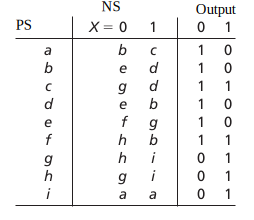
\includegraphics[width=0.3\linewidth]{./media/15.15-state-table.png}
  \label{p:state-reduction}
\end{prob}
\newpage

\begin{prob}
  % Reduce the following state table to a minimum number of states using
  % implication charts (20 marks).
  \begin{enumerate}
  \item
    Use the guideline method (Highest priority and Medium priority only) to determine a suitable \textbf{state assignment} for the state table (20 marks).
  % % \item
  % % Realize the table using D flip-flops.
  \item Realize the table using J-K flip-flops (30 marks).
  \end{enumerate} 

  \begin{tabular}{c|cc|c}
    \toprule
    Present State & \multicolumn{2}{c|}{Next State} & Output (Z)\\
                  & X = 0 & 1 & \\
                  \midrule
    A & A & B & 1\\
    B & C & E & 0\\
    C & F & G & 1\\
    D & C & A & 0\\
    E & B & G & 1\\
    F & F & B & 1\\
    G & C & F & 0\\
    \bottomrule
  \end{tabular}
\end{prob}
\newpage

\begin{prob}
  A 4:2 priority encoder takes 4 inputs $y_0, y_1, y_2, y_3$ and has three outputs, $w_1, w_0$ and $\text{IST}$. Find boolean expressions for $w_1$ and $w_0$ using K-maps for the priority encoder. The priority encoder truth table is given for reference (``*'' indicates all possible input combinations and ``d'' indicates don't care output). (10 marks) \\
  \begin{tabular}{cccc|ccc}
    \toprule
    \multicolumn{4}{c|}{Inputs} & \multicolumn{3}{c}{Outputs}\\
    $y_0$ & $y_1$ & $y_2$ & $y_3$ & $w_1$ & $w_0$ & $\text{IST}$ \\
    \midrule
    0 & 0 & 0 & 0 & d & d & 0\\
    1 & * & * & * & 0 & 0 & 1\\
    0 & 1 & * & * & 0 & 1 & 1\\
    0 & 0 & 1 & * & 1 & 0 & 1\\
    0 & 0 & 0 & 1 & 1 & 1 & 1\\
    \midrule
  \end{tabular}
\end{prob}
\newpage

\begin{prob}
  % 9 study guide 5
  (Optional for extra credit) The following diagram shows the pattern of 0’s and 1’s stored in a ROM
  with eight words and four bits per word. What will be the values of $F_1 , F_2 ,
  F_3 , and F_4$ if $A= B = 0$ and $C = 1$?
  Also give the minterm expansions for $F_1$ and $F_2$ (20 marks).\\
  \includegraphics[width=0.4\linewidth]{./media/ROM-minterms.png}
\end{prob}
\newpage

